\documentclass{beamer}
\usepackage[utf8]{inputenc}

\usepackage{graphicx}

\usetheme{Madrid}
%\usetheme{boxes}
%\usetheme{Singapore}
%\usetheme{Pittsburgh}

\usecolortheme{whale}
%\usecolortheme{dove}
%\usecolortheme{lily}
\usecolortheme{orchid}

\title{An educational kernel for the Raspberry Pi}
\subtitle{CS310 - Presentation}
\author{Thomas Archbold}
\date{\today}

\begin{document}

\begin{frame}
    \titlepage
\end{frame}

\begin{frame}{Introduction}
\centering
    Operating systems are some of the most pervasive pieces of software around,
    but also some of the most complex \\~\\

    The introduction of the Raspberry Pi has made computers much more accessible
    - allows and encourages experimenting at all levels \\~\\

    There are several official operating systems for the Pi - NOOBS, Raspbian,
    Windows IoT core, PiNET - but none provide a resource to learn about the
    operating system itself

    \begin{figure}
        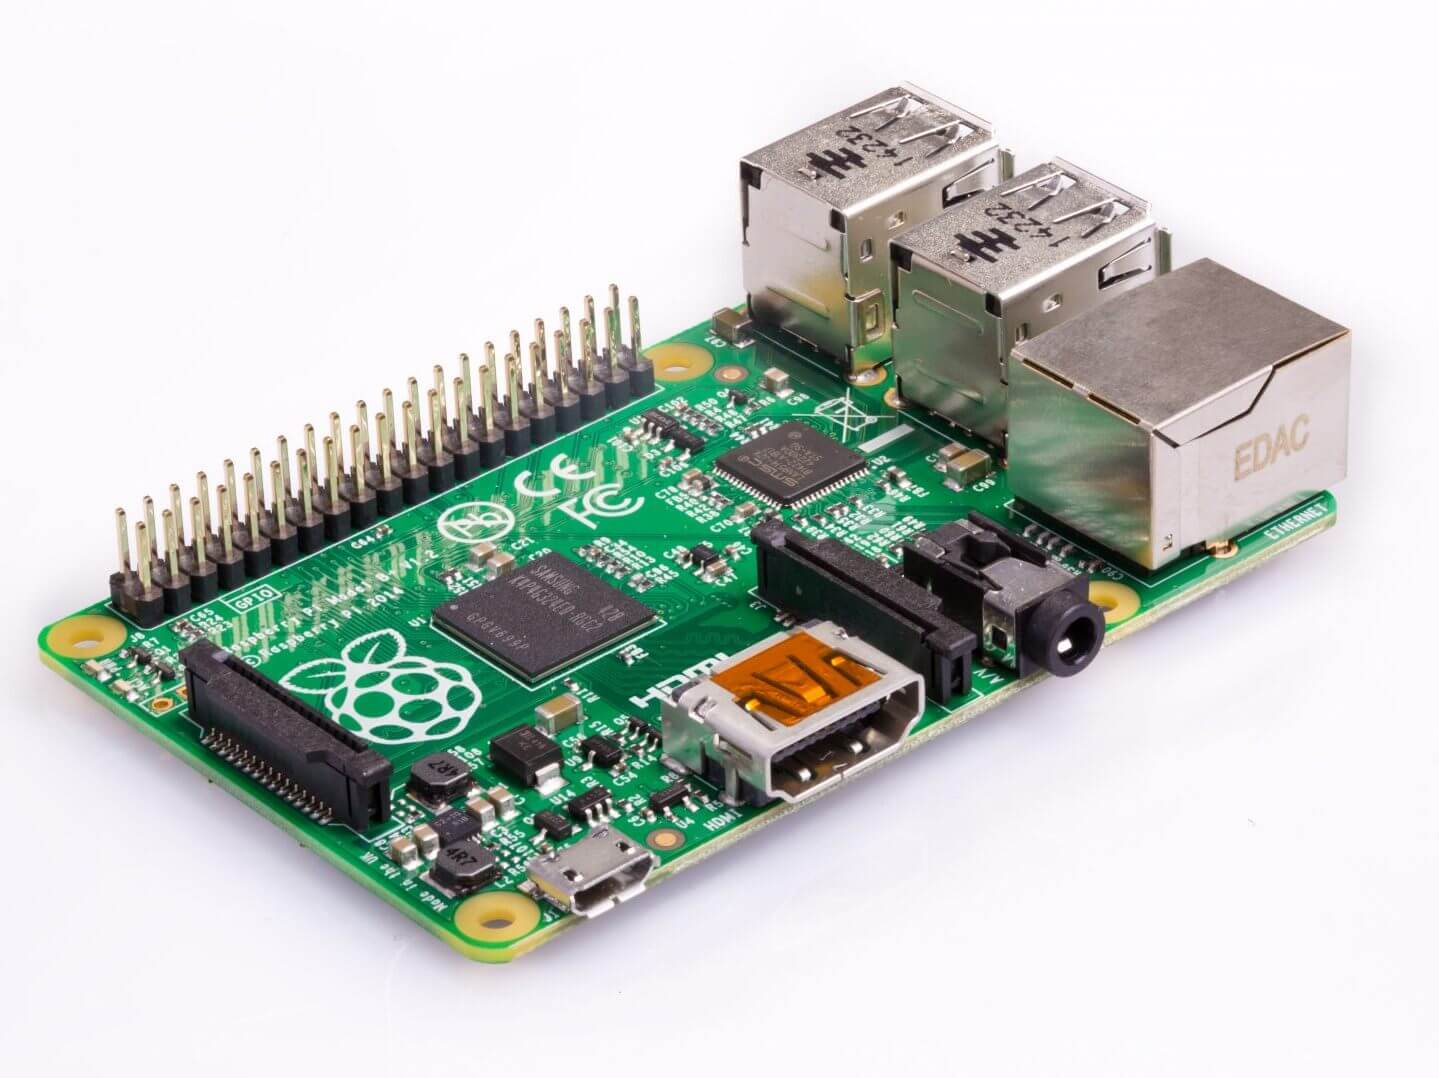
\includegraphics[width=0.4\linewidth]{raspi1B.jpg}
    \end{figure}
\end{frame}

\begin{frame}{Objectives}
    \textbf{Main goal:}
    to write a configurable operating system for the Raspberry Pi capable on
    booting on real hardware for educational and hobbyist use. \\~\\

    Specifically, this involves:
    \begin{itemize}
        \item providing different approaches for tasks such as scheduling,
            interprocess communication, and permanent storage
        \item allowing the user to configure the system at compile time to use
            different combinations of these approaches, and
        \item exposing a simple and easily extensible interface for additional
            features
    \end{itemize}
\end{frame}

\begin{frame}{Background material}
    \begin{itemize}
        \item Pintos - Stanford's instructional x86 operating system, used to
            teach their CS140 course
        \item Baking Pi - Cambridge's tutorial on writing an operating system
            for the Raspberry Pi in assembly
        \item MINIX - Tanenbaum and Woohull's illustrative operating system for
            ``Operating Systems: Design and Implementation''
        \item The little book about OS development - Helin and Renberg's
            ``practical guide to writing your own x86 operating system''
    \end{itemize}
\end{frame}

\begin{frame}{Why is this project worthwhile?}
\centering
    It is more difficult to get into low-level/systems programming $\Rightarrow$
    focus is on clear code to aid understanding as much as possible \\~\\

    The project attempts to demystify aspects of operating system development -
    able to see the theory in practise \\~\\

    Will provide an accessible platform to further tinker and experiment with
    operating system development, with little to lose
\end{frame}

\begin{frame}{Useful concepts - compilation}
    \textbf{Operating System} \\~\\
    \textbf{Freestanding environment} \\~\\
    \textbf{Cross-compiler} \\~\\
    \textbf{Linker} \\~\\

\end{frame}

\begin{frame}{Useful concepts - general OS concepts}
    \textbf{Kernel} \\~\\
    \textbf{Exception} \\~\\
    \textbf{Interrupt Request (IRQ)} \\~\\
    \textbf{Process} \\~\\
    \textbf{Concurrency} \\~\\
    \textbf{Context Switch} \\~\\
    \textbf{Synchronisation} \\~\\
    \textbf{Interprocess Communication} \\~\\
\end{frame}

\begin{frame}{Tools used}
    Languages: C and ARM assembly \\~\\
    Cross-compiler toolchain: \texttt{arm-none-eabi} \\~\\
    Build automation: Make \\~\\
    Version control: git \\~\\
    Emulation: QEMU \\~\\
    Model: Raspberry Pi 1 Model B+
\end{frame}

\begin{frame}{Project management}

\end{frame}

\begin{frame}{Design overview}

\end{frame}

\begin{frame}{Next steps}

\end{frame}

\begin{frame}{Conclusions}

\end{frame}

\end{document}

